% Chapter 5 from the standard thesis template
%   with a full page figure and a sideways table.

%Chapter 5 will look at the results from the experiments and how the performance of the new software defined radiometer measured up.

\chapter{RESULTS AND ANALYSIS}

Radiometers measure power and it is this information that we can use to determine information about a certain target.  This power however is often expressed in terms of an equivalent temperature and if we are looking at an object, this is the brightness temperature of that object.  The primary function of the radiometer is to measure the power that is seen at the radiometer's antenna.  Ideally this is the brightness temperature of an object of interest.  In our case, this is usually looking at the ground or soil sample.  Thus the goal of the radiometer is to measure this antenna temperature with sufficient resolution and accuracy that a correlation can be made between the antenna temperature and the object's temperature that we are studying.

\section{Performance of a radiometer}
The performance of a radiometer can be measured by looking at both the sensitivity and the accuracy of the radiometer.  In addition, we need to be concerned with the stability of the radiometer as this affects the accuracy of the radiometer.


\subsection{Sensitivity}
Sensitivity of the radiometer relates to the amount of power that the radio selects from the antenna.  This selection is then dependent on the bandwidth that the radiometer is able to listen to.  The radiometer however detects not only the signal of interest but also receives a noise signal as well.  This noise is added to the signal and can not be separated from the signal.  Because this noise is added to the signal, we must be able to determine a change in the signal while the noise signal is also present.  

Power from the radiometer can be expressed in equation \ref{eq:final_power} from chapter 2, where we take into consideration bandwidth, gain and the input from the antenna plus the noise added from the antenna.  

Sensitivity relates to being able to distinguish one signal from the other.  In other words, we must be able to distinguish, or detect, our wanted signal from noise that is present in the signal.  To demonstrate this, consider a system that has a system noise temperature of 700K and an antenna temperature of 300K.  This gives us a total noise temperature of 1000K.  Therefore, if we wish to detect a change of 1K, we need to be able to detect between 1000K and 1001K.

Since our signal is really random fluctuations about a mean power input to our system, we can reduce the fluctuations by averaging or integrating the signal.  This results in equation \ref{eq:rad_sensitivity} which is derived in chapter 2.

\begin{equation} \label{eq:rad_sensitivity}
\Delta T=\frac{T_{A}+T_{N}}{\sqrt{\beta * \tau}}
\end{equation}


This equation gives us the radiometer sensitivity based on the input, which is both the noise and input signal with consideration to the bandwidth and integration time, or averaging, that is done to the signal.  

\subsection{Accuracy and Stability}
Stability and accuracy are additional problems that need to be considered when looking at the radiometer system.  To begin we can once again look at the power received equation that we discussed in Chapter 2 and is equation \ref{eq:final_power}.

As we look at this equation, we can see that if k, B, G, and $T_{N}$ are constant, then stability can be assured.  k is a known constant and we can also assume that our bandwidth, $\beta$, will also remain constant.  Gain and the noise temperature however will vary.  

Gain is usually our largest factor that can change on a radiometer and even with a software defined radio this is still a large source of variation.  This is due to the analog nature of the amplifiers that affect a large portion of the gain in our system.  Various things can affect our gain but the two largest factors is the physical temperature of the amplifier and the voltage that feeds the amplifier.  Voltage can be controlled to a degree.  High accuracy voltage regulators can help control fluctuations in voltages that can in turn affect the gain.  A factor however that is harder to control is temperature.  It can be seen in equation \ref{eq:rad_stability} that temperature change due to gain fluctuations us directly related to the changes in gain and the overall gain of the system. It is because of this that the current ISU radiometer has gone to great strides to control the temperature of the amplifiers to maintain a constant temperature.

\begin{equation} \label{eq:rad_stability}
\Delta T_G=T_{sys} \left(\frac{\Delta G}{G}\right)
\end{equation}

To verify stability of the radiometer, we look to see how much change the radiometer records over a relative long period of time.  To test this a matched load was submerged in a liquid nitrogen bath for an extended period of time, in this case for fifteen minutes.  The readings were then looked at to study the trend of the data.  The data is graphed in figure \ref{Stability}.

\begin{figure}[h!tb] \centering
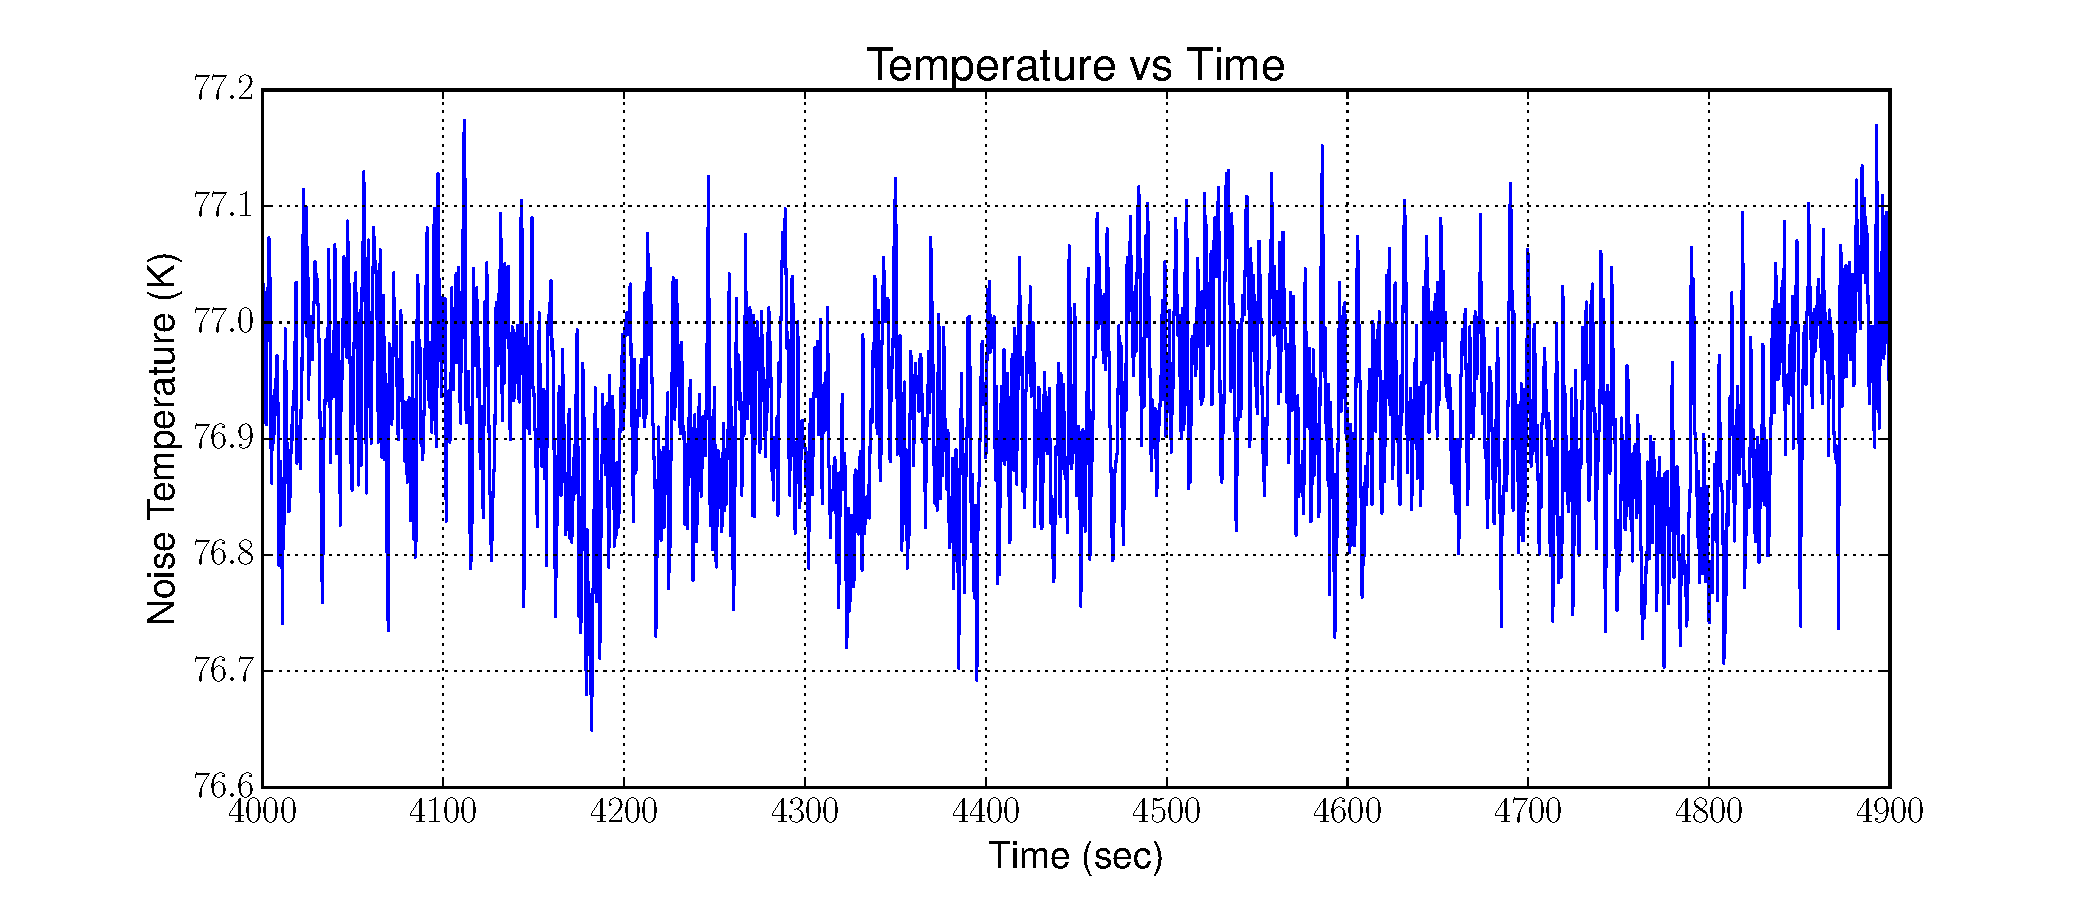
\includegraphics[width=\textwidth]{Experiments/Exp2/sdr_calibrated_zoom.pdf}
\isucaption{Graph of the calibrated total power over a period of fifteen minutes.}
\label{Stability}
\end{figure}

\begin{figure}[h!tb] \centering
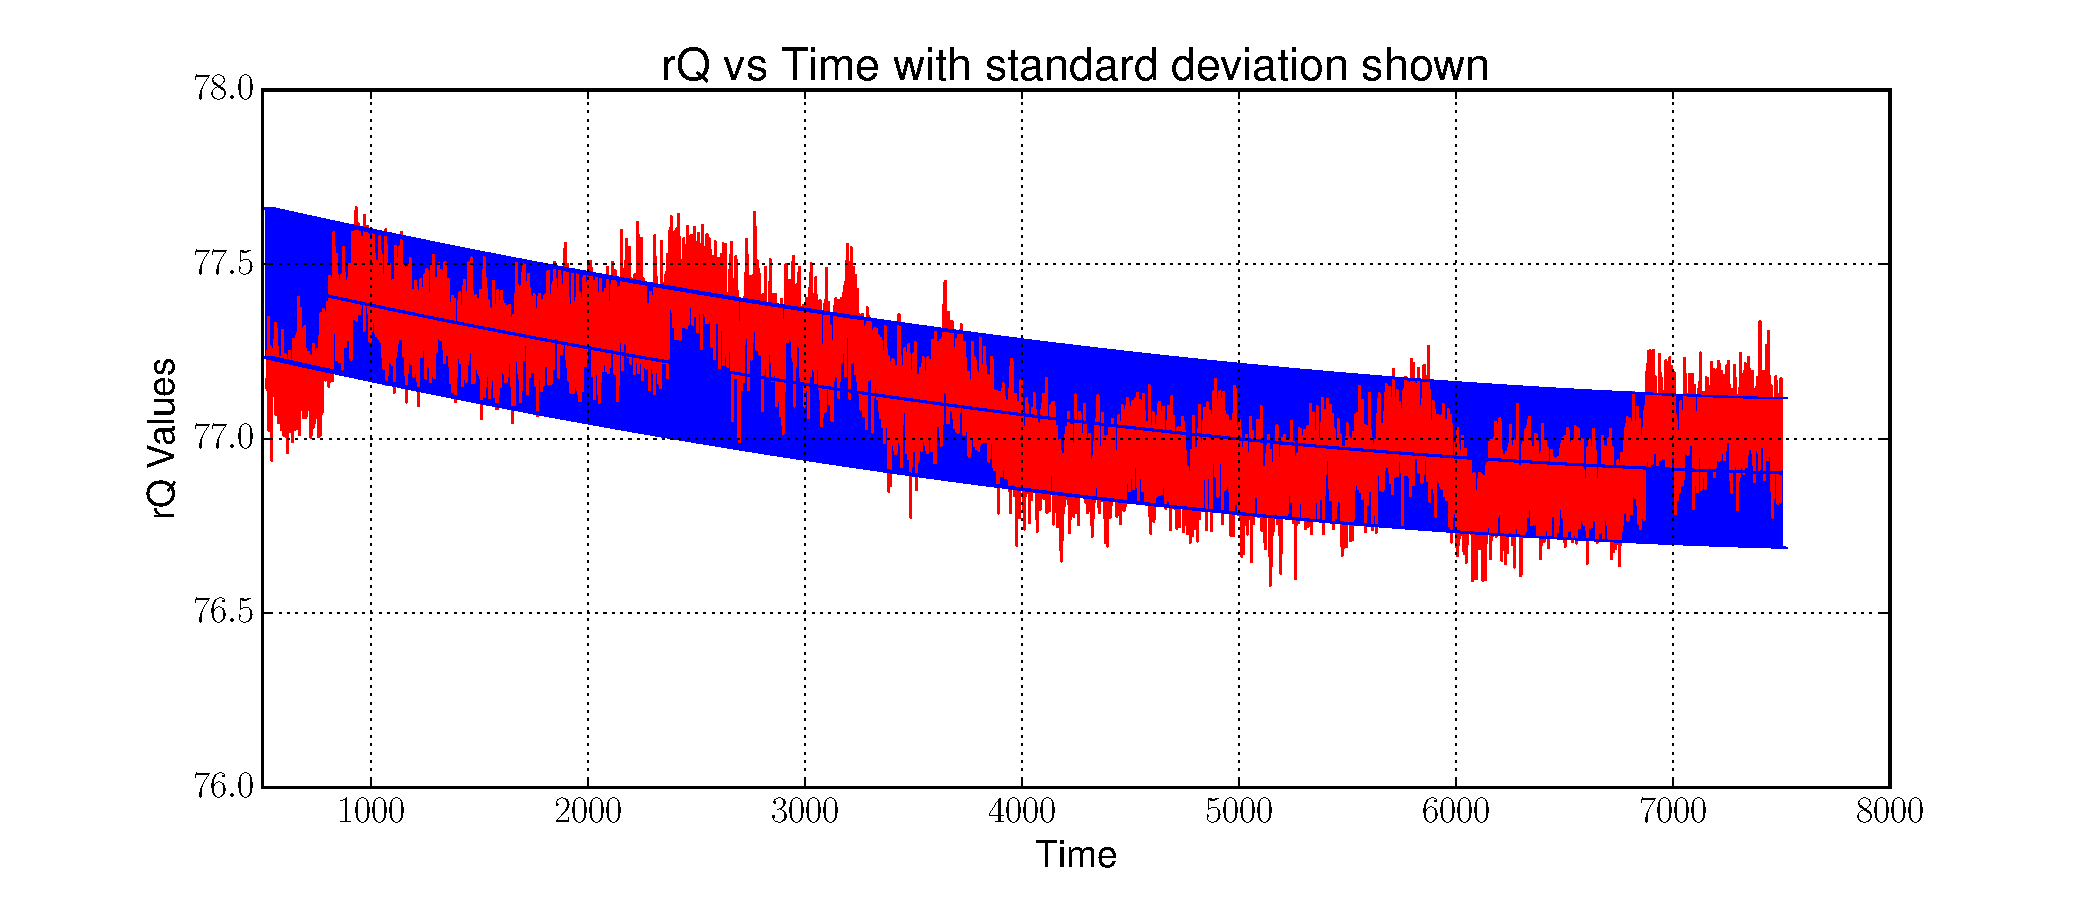
\includegraphics[width=\textwidth]{Experiments/Exp2/calib_vstime_stddev.pdf}
\isucaption{Graph of the calibrated total power with the standard deviation plotted.}
\label{Stability_calib}
\end{figure}

As it can be seen in figure \ref{Stability}, the amount of change over a period of one hour is quite small.  The standard deviation for this sample is 0.09 kelvin.  The $NE\Delta T$ calculated using 10 MHz for the bandwidth, an integration time of 2 seconds and with our sample at 77 Kelvin is calculated to be 0.10 Kelvin with a system temperature of 350 Kelvin.  Therefore our system is behaving as we expect it to for this stability test.

Figure \ref{Stability_calib} shows a graph of the total readings but with the standard deviation now plotted.  This shows that the system is stable and is operating as expected within our expected $NE\Delta T$.

\section{Required Performance Requirements}

To help us quantify the required performance of the radiometer, we referred to information provided to us by Dr. Brian Hornbuckle but also derived from existing radiometers.  As stated earlier, although a radiometer measures power, we often convert this to an equivalent brightness temperature.  Specifically, we are looking at the brightness temperature of the antenna added to the brightness temperature of the object of interest.  We also have to be able to detect a minimum amount of power.  Since changes in noise can be small, the better the sensitivity of the radiometer, the better we can detect these small changes.  

The requirements given are outlined in the table below.

\begin{table}[h!tb] \centering
\isucaption{Required Radiometer performance}
\label{rad_performance}
% Use: \begin{tabular{|lcc|} to put table in a box
\begin{tabular}{lcc} \hline
\textbf{Parameter} & \textbf{Value} & \textbf{Units} \\ \hline
Minimum bandwidth & 20 & MHz \\
Operational frequency & 1400 - 1420 & MHz \\
$NE\Delta T$ & 1 & Kelvin \\ \hline
\end{tabular}
\end{table}

\section{Square-law Detector Performance}
The Square-law detector was added to our system in order to give us another reference point and to help verify the power output that the software defined radio.  The performance of our square-law detector is based on two items.  The first is the actual square-law detector itself.  The sensitivity of this device accounts for most of the performance factor of the system.  In our system the output of this square-law detector is then feed directly into an analog to digital converter.  Therefore the performance of this A/D converter needs to be accounted for as well [\cite{Terlep}].  

For our square-law detector, it has a noise output of $25nV/ \sqrt{Hz}$ at 100 kHz and will detect a signal as low as $-60$ dBm.  This works will with our needs since the RF front end brings the noise floor to approximately $-30$ dBm.


\section{Software Defined Radio Performance}
Performance of the software defined radio is governed by the system that takes in the RF signal and then digitizes the signal.  Once the signal is in digital form, we no longer are concerned about loss of performance due to additional noise that may get added to the system.  For this reason, we attempt to digitize the signal as soon as possible.

For the N200 this is done by the DBSRX2 daughter-board that plugs into the N200 base system.  While this board does play a part in the overall system performance, because this sits later in the chain however the impact to the performance is low as shown in equation \ref{noise_factor}.  However, this module does need to be in the frequency range of the radiometer, or in our case 1.4 GHz.  This board meets that criteria.  Ideally, we still want the noise figure on this board as low as possible, even though the impact is low.  The DBSRX2 does meet this having a noise figure of approximately 5 dBm.
\section{Benefits to Software Defined Radio Radiometer}
A study was conducted on what benefits a software defined radio radiometer would have over a more traditional radiometer.  This was focused on looking at three main areas; cost, weight and size, and the value a SDR radiometer can add over traditional radiometers.

\subsection{Cost Benefits}
Software defined radios have become more commonplace in recent years and this has generated a number of COTS solutions.  A COTS solution is often a lower cost solution due to the mass manufacturing that takes place.  This has driven the cost of many SDRs to under one thousand dollars while still having excellent performance characteristics.  The N200 SDR purchased for this research cost fifteen hundred dollars and the daughter-board cost one hundred and fifty dollars approximately.  Many other software defined radios however have come out on the market since then.  Ettus for example has some that are below one thousand dollars and the author has also obtained the HackRF One SDR that now sells for three hundred dollars.  The main difference with these software defined radios is with both the resolution, or how many bits the ADC is, and the bandwidth they are able to handle.

\begin{table}[h!tb] \centering
\isucaption{Cost Analysis}
\label{cost_table}
% Use: \begin{tabular{|lcc|} to put table in a box
\begin{tabular}{lcc} \hline
\textbf{Device} & \textbf{Quantity} & \textbf{Cost} \\ \hline
\textbf{SDR Solution}& & \\ \hline
N200 SDR & 1 & \$1515 \\
LNA at \$60 ea. & 3 & \$180 \\
DBSRX2 Daughter-board & 1 & \$152 \\
GNURadio & 1 & \$0 \\ \hline
Total & & \$1847 \\ \hline
\textbf{ISU Radiometer} \\ \hline
LNA, FPGA, ADC, Microcontroller and power supplies & 1 & \$10,000\tablefootnote{Purchase price in 2005} \\ \hline
\textbf{Commercial Off the Shelf Unit}\\ \hline
Spectracyber 1420 MHz Hydrogen Line Spectrometer & 1 & \$2,650 \\ \hline

\end{tabular}
\end{table}

As see in table \ref{cost_table}, even the higher cost Ettus research equipment is a lower cost option than the custom built ISU radiometer purchased from University of Michigan and even a comparable off the shelf radiometer.  It should be noted that the radiometer from the University of Michigan is also a dual polarization radiometer so there are two RF front ends and two ADCs that feed into a FPGA board.  It would be quite easy to add dual polarization to the Ettus N200 SDR as it does support two daughter-boards.  This would increase the cost to \$2,179 for the additional LNAs and daughter-board.

The largest cost benefit is that key components that you find in a radiometer, the filters and square-law detector can now be all done in software instead of needed additional equipment.  The system is also much more frequency agile, which means it can work on a broader range of frequencies than most traditional radiometers with very little change in hardware and in some cases may require no change in hardware.  Some of this does depend on the SDR hardware however.  The Ettus N200 for example uses daughter-boards to provide the RF interface.  While these boards provide a high quality in the RF signal, it does come at a cost and are usually designed for certain bands of frequencies.  Other low cost SDRs however are also very wide range in the frequencies they will work in.  The HackRF for example works from 10 MHz to 6 GHz, but does so at the cost of lower resolution, less gain in its front end and a lower bandwidth that it can handle.

\subsection{Weight and component size benefits}

A typical radiometer has many components that are involved in the design of the radiometer.  This includes filters, LNAs and the power detection or square-law detector used.  These components add both weight, size and costs to the radiometer.  A software defined radio however digitizes the signal and we are able to replace the filters and square-law detector with their software equivalent.  While a software defined radio does add both the ADC and usually a FPGA to do the processing on the signal, advances in semiconductor technology has continued to shrink these components.  These components are also lighter than the filters often used in radiometers.

\begin{table}[h!tb] \centering
\isucaption{Weight Analysis}
\label{weight_table}
% Use: \begin{tabular{|lcc|} to put table in a box
\begin{tabular}{lc} \hline
\textbf{Device} & \textbf{Mass} \\ \hline
\textbf{SDR Solution} & \\ \hline
N200 SDR & 1.2 kg \\
LNA at .03 kg ea & .09 kg \\
DBSRX2 Daughter-board & .1 kg \\ \hline
Total & 1.39 kg \\ \hline
\textbf{ISU Radiometer} \\ \hline
LNA, FPGA, ADC, Microcontroller and power supplies & 22.7 kg \\ \hline
\textbf{Commercial Off the Shelf Unit}\\ \hline
Spectracyber 1420 MHz Hydrogen Line Spectrometer & 6 kg\tablefootnote{Estimated, no data available} \\ \hline

\end{tabular}
\end{table}

Size is another benefit as since semiconductor technology has continued to shrink components.  Again, since items like the filters and square-law detector are removed and done in software this helps to reduce the overall size.  

\subsection{Value added benefits}

A software defined radio radiometer adds additional value for two reasons.  One, it is able to work with both frequency and magnitude where most radiometers do not.  This allows for additional analysis on the signal and can help identify issues such as an interfering signal that was demonstrated in this thesis.  

Second, we are able to have an agile system that is able to adapt to changing conditions with very little or no change to hardware.  Different types of radiometers can be implemented such as a Dicke radiometer, dual polarization radiometer or a radiometer that can perform Stokes parameters.  In addition, since we have both frequency and power information we can create a system that is able to adapt to changing conditions such as dealing with an interfering signal.  

\section{Disadvantages of a SDR Radiometer}
Although we have outlined a number of advantages of using a COTS SDR Radiometer and how a SDR can add additional value to the radiometer system, there are some disadvantages to a SDR Radiometer.

\subsection{Power Consumption}
One of the largest drawbacks to a SDR radiometer can be in the power consumption of the SDR.  With the move to perform functions such as power detection and filtering we now require additional computational power to perform these tasks.  With those computational cycles additional power is now required.  The use of FPGAs and SoC however can help to minimize these power concerns as they are more efficient than using a full scale x86 based processor and on board computer system.  

Power and CPU requirements also increase as we add additional functionality such as filtering an offending signal.  While these additions may not require additional hardware, it can require additional processor or computational requirements.  This will cause additional strain on the processor and also in the memory requirements for the SDR as well.

\subsection{Bandwidth constraints}
While SDR technology has advanced, bandwidth is still a constraint that affects SDRs and in turn a SDR Radiometer.  Bandwidth plays a critical role in the radiometers sensitivity as explained in this thesis, therefore the fact that many SDRs are limited in bandwidth does create a disadvantage.  In many cases this bottle neck takes place in both the transport and processing of large bandwidth systems.  This also relates to the power consumption disadvantage since larger bandwidth also means requiring additional computational cycles as well.  

In contrast, a square-law detector usually has a very large bandwidth, as much as one gigahertz, and is why we usually need to filter to the frequency band of interest.  